\documentclass[12pt, a4paper, oneside]{Thesis} % Paper size, default font size and one-sided paper
\usepackage{wrapfig}
\usepackage{lscape}
\usepackage{rotating}
\usepackage{graphicx}
\usepackage{caption}
\usepackage{amsmath}

\usepackage{lineno,hyperref}
\modulolinenumbers[5]

\usepackage{amssymb}
\usepackage{graphicx}
\usepackage{array}
\usepackage{float}
\usepackage{placeins}
\usepackage{stackengine}
\usepackage{url}
\usepackage{numprint}
\usepackage{caption}

\usepackage{booktabs}  
\usepackage{siunitx}
%\usepackage[showframe=false]{geometry}
\usepackage{subfigure}

\usepackage{listings}
\lstset{breaklines=true}
\lstset{basicstyle=\small\ttfamily\singlespacing}

\nprounddigits{3}
\newcolumntype{P}[1]{>{\centering\arraybackslash}p{#1}}
\newcolumntype{M}[1]{>{\centering\arraybackslash}m{#1}}

\setstackEOL{\#}
\setstackgap{L}{12pt}


%\usepackage{subcaption} %incompatible with subfig
\graphicspath{{Pictures/}} % Specifies the directory where pictures are stored
\usepackage{natbib} % Use the natbib reference package - read up on this to edit the reference style; if you want text (e.g. Smith et al., 2012) for the in-text references (instead of numbers), remove 'numbers' v

\hypersetup{urlcolor=black, colorlinks=false} % Colors hyperlinks in blue - change to black if annoyingv`	

\thesistitle{Latency Analysis in Serverless Architectures}
\supervisor{Prof. Sandip Chakraborty}
\degree{Master of Technology}
\degreemajor{Computer Science and Engineering}
\authors{Nishant Baranwal Somy}
\rollno{15CS30044}
\university{Indian Institute of Technology Kharagpur}
\department{Department of Computer Science and Engineering}
\unisite{http://www.iitkgp.ac.in}
\depsite{http://www.cse.iitkgp.ac.in}
\placeshrt{Kharagpur}
\placelng{Kharagpur - 721302, India}
\datesub{November 14, 2019}
\datesig{November 14, 2019}
\semsub{Autumn Semester, 2019-20}
%\keywords{Steel Structure}
\coursecd{Project-I (CS57003) }

\title{\ttitle} % Defines the thesis title - don't touch this
\begin{document}
%\makeatletter
%\renewcommand*{\NAT@nmfmt}[1]{\textsc{#1}}
%\makeatother

% prints author names as small caps


\frontmatter % Use roman page numbering style (i, ii, iii, iv...) for the pre-content pages

\setstretch{1.6} % Line spacing of 1.6 (double line spacing)

% Define the page headers using the FancyHdr package and set up for one-sided printing
\fancyhead{} % Clears all page headers and footers
\rhead{\thepage} % Sets the right side header to show the page number
\lhead{} % Clears the left side page header

%\pagestyle{fancy} % Finally, use the "fancy" page style to implement the FancyHdr headers

\newcommand{\HRule}{\rule{\linewidth}{0.5mm}} % New command to make the lines in the title page

% PDF meta-data
\hypersetup{pdftitle={\ttitle}}
\hypersetup{pdfsubject=\subjectname}
\hypersetup{pdfauthor=\authornames}
\hypersetup{pdfkeywords=\keywordnames}

%----------------------------------------------------------------------------------------
%	TITLE PAGE
%----------------------------------------------------------------------------------------
\maketitle
%\titlepg % Add a gap in the Contents, for aesthetics

\clearpage % Start a new page

%----------------------------------------------------------------------------------------
%	DECLARATION PAGE
%	Your institution may give you a different text to place here
%----------------------------------------------------------------------------------------


\Declaration% Add a gap in the Contents, for aesthetics


%----------------------------------------------------------------------------------------
%	CERTIFICATE PAGE
%----------------------------------------------------------------------------------------

\addtotoc{Certificate} % Add the "Abstract" page entry to the Contents

\certificate{\addtocontents{toc}{} % Add a gap in the Contents, for aesthetics

}

\clearpage % Start a new page

%----------------------------------------------------------------------------------------
%	ABSTRACT PAGE
%----------------------------------------------------------------------------------------

%\addtotoc{Abstract} % Add the "Abstract" page entry to the Contents

%\abstract{\addtocontents{toc}{} % Add a gap in the Contents, for aesthetics

%Enter content here. 
%}

%\clearpage % Start a new page



%----------------------------------------------------------------------------------------
%	ACKNOWLEDGEMENTS
%----------------------------------------------------------------------------------------

%\setstretch{1.3} % Reset the line-spacing to 1.3 for body text (if it has changed)

%\acknowledgements{\addtocontents{toc}{}%\vspace{1em}} % Add a gap in the Contents, for aesthetics

%Enter acknowledgement content here.

%}
%\clearpage % Start a new page

%----------------------------------------------------------------------------------------
%	LIST OF CONTENTS/FIGURES/TABLES PAGES
%----------------------------------------------------------------------------------------

\pagestyle{fancy} % The page style headers have been "empty" all this time, now use the "fancy" headers as defined before to bring them back

\lhead{\emph{Contents}} % Set the left side page header to "Contents"
\tableofcontents % Write out the Table of Contents

%\lhead{\emph{List of Figures}} % Set the left side page header to "List of Figures"
%\listoffigures % Write out the List of Figures

%\lhead{\emph{List of Tables}} % Set the left side page header to "List of Tables"
%\listoftables % Write out the List of Tables

%----------------------------------------------------------------------------------------
%	ABBREVIATIONS
%----------------------------------------------------------------------------------------

% \clearpage % Start a new page

% \setstretch{1.5} % Set the line spacing to 1.5, this makes the following tables easier to read

% \lhead{\emph{Abbreviations}} % Set the left side page header to "Abbreviations"
% \listofsymbols{ll} % Include a list of Abbreviations (a table of two columns)
% {
% \textbf{FEA} & \textbf{F}inite \textbf{E}lement \textbf{A}nalysis \\
% \textbf{FEM} & \textbf{F}inite \textbf{E}lement \textbf{M}ethod \\
% \textbf{LVDT} & \textbf{L}inear \textbf{V}ariable \textbf{D}ifferential \textbf{T}ransformer \\
% \textbf{RC} & \textbf{R}einforced \textbf{C}oncrete
% %\textbf{Acronym} & \textbf{W}hat (it) \textbf{S}tands \textbf{F}or \\
% }

%----------------------------------------------------------------------------------------
%	PHYSICAL CONSTANTS/OTHER DEFINITIONS
%----------------------------------------------------------------------------------------
%
%\clearpage % Start a new page
%
%\lhead{\emph{Physical Constants}} % Set the left side page header to "Physical Constants"
%
%\listofconstants{lrcl} % Include a list of Physical Constants (a four column table)
%{
%Speed of Light & $c$ & $=$ & $2.997\ 924\ 58\times10^{8}\ \mbox{ms}^{-\mbox{s}}$ (exact)\\
%% Constant Name & Symbol & = & Constant Value (with units) \\
%}

%----------------------------------------------------------------------------------------
%	SYMBOLS
%----------------------------------------------------------------------------------------

% \clearpage % Start a new page

% \lhead{\emph{Symbols}} % Set the left side page header to "Symbols"

% \listofnomenclature{lll} % Include a list of Symbols (a two column table)
% {
% $D^{el}$ & elasticity tensor \\
% $\sigma$ & stress tensor \\
% $ \varepsilon $ & strain tensor \\
% % Symbol & Name & Unit \\

% }

%----------------------------------------------------------------------------------------
%	DEDICATION
%----------------------------------------------------------------------------------------
%
%\setstretch{1.3} % Return the line spacing back to 1.3
%
%\pagestyle{empty} % Page style needs to be empty for this page
%
%\dedicatory{For/Dedicated to/To my\ldots} % Dedication text
%
%\addtocontents{toc}{\vspace{2em}} % Add a gap in the Contents, for aesthetics

%----------------------------------------------------------------------------------------
%	THESIS CONTENT - CHAPTERS
%----------------------------------------------------------------------------------------

\mainmatter % Begin numeric (1,2,3...) page numbering

\pagestyle{fancy} % Return the page headers back to the "fancy" style

% Include the chapters of the thesis as separate files from the Chapters folder
% Uncomment the lines as you write the chapters

% Introduction - 
% Background : Requirement of serverless, its pros and cons

% Chapter Template

\chapter{Introduction} % Main chapter title

\label{Chapter 1} % Change X to a consecutive number; for referencing this chapter elsewhere, use \ref{ChapterX}

\lhead{Chapter 1. \emph{Introduction}} % Change X to a consecutive number; this is for the header on each page - perhaps a shortened title

%----------------------------------------------------------------------------------------
%	SECTION 1
%----------------------------------------------------------------------------------------

In the current web service age, the deployment of services in off premises is more easy task. The users not even need to estimate their server specifications during the Service Level Agreement (SLA) negotiation. This can be possible by the concept of serverless application or Function as a Service (FaaS) \cite{Wang_usenix_2018}. Popular cloud providers such as Amazon, Microsoft, and Google already introduced their serverless solutions as AWS Lamda\footnote{https://aws.amazon.com/lambda/}, Azure Function\footnote{https://azure.microsoft.com/en-in/solutions/serverless/}, and Google Cloud Function\footnote{https://cloud.google.com/functions/} respectively. Apart from these big players, some new solutions has also started providing the FaaS service \cite{servelless_online_2019}.

\noindent Serverless applications are flexible enough to focus on user's core product and business logic instead of responsibilities like operating system (OS) access control, OS patching, provisioning, right-sizing, scaling, and availability \cite{Lloyd_2018}. By building your application on a serverless platform, the platform manages these responsibilities for you. These new concepts are providing the following capabilities:
\begin{itemize}
	\item \textbf{No server management:} Users need not to provision or maintain any servers. There is no software or runtime to install, maintain, or administer.
	\item \textbf{Flexible scaling:} Users can scale their application automatically or by adjusting its capacity through toggling the units of consumption (for example, throughput, memory etc.) rather than units of individual servers.
	\item \textbf{High availability:} Serverless applications have built-in availability and fault tolerance. Useres not need to architect for these capabilities because the services running the application provide them by default.
	\item \textbf{No idle capacity:} Users need not to pay for idle capacity. There is no need to pre-provision or over-provision capacity for things like compute and storage. There is no charge when your code is not running.
\end{itemize}

%\begin{figure}[!ht]
%	\centering
%	\includegraphics[width=0.5\linewidth, height=0.8\columnwidth]{image/serverless_arch.eps}
%	\caption{Serverless Architecture}\label{fig:serverless_arch}
%\end{figure} 

%\subsection{Some popular serverless usecasess and their archtechture:}
Currently, most of the technology adopters are startups who seek for a possibility to scale painlessly and to lower the entrance barrier. Serverless is also a perfect approach for applications that do not run continuously but rather have quiet periods and peaks of traffic. This concept can be useful for a wide range of applications, from a simple database (DB) application to complex data analytics pipeline applications \cite{Bhattacharjee_USENIX_2019}.
%\begin{enumerate}
%	\item \textbf{Simple DB appliacation:} For any small scale application such as iteractive web site, ERP solutions etc. Serverless is a good candidate to opt as a deployment technology. Figure \ref{fig:simpleDB_serverless} illustrate a simple DB application.
%	
%	\item \textbf{Data analytics pipeline:}
%	\cite{Bhattacharjee_USENIX_2019}.
%\end{enumerate}
% 

%Related work
In the literature, a few recent works have significantly explored serverless computing from different perspectives. In \cite{Akkus_Sand_Usenix_2018}, a new serverless computing system that provides lower latency, better resource efficiency and more elasticity than existing serverless platforms is discussed. To achieve these properties, authores have introduced a model SAND, based on application-level sandboxing and an hierarchical message bus. Here, the design and implementation of SAND, as well as experience in building and deploying serverless applications on it are presented. In \cite{Oakes_USENIX_2018}, the author has analyzed Linux container primitives, identifying scalability bottlenecks related to storage and network isolation where there is a container system optimized for serverless workloads. Based on these findings, they have implemented SOCK, a container system optimized for serverless workloads model. They have identified container initialization and package dependencies as common causes of slow Lambda startup. In \cite{Hong_USENIX_2018}, author has advocated for taking a serverless approach by proposing six serverless design patterns to build security services in the cloud. For each design pattern, they describe the key advantages and present applications and services utilizing the pattern. Using the proposed patterns as building blocks, they have introduced a threat intelligence platform that collects logs from various sources,  alerts malicious activities, and takes actions against such behaviors.

%%\cite{Ishakian_2018}.

Though advantageous in focusing on the user's business logic rather than the platform management, serverless architectures has latency related issues as it is stateless and need to communicate with data source, other serverless functions. In this paper, we analyze this latency of serving requests for different serverless architectures. First, we take the simplest use case of a database application and compare the performance with the traditional VM based approach. Next, we analyze a more complex data pipeline involving multiple functions and observe how it impacts the overall latency of the service. Then, we propose some simple caching strategies to improve the response times. Finally, we discuss their pitfalls.
\section{What is Cloud Computing?}

Cloud computing is an internet-based computing service in which large groups of remote servers are
networked to allow centralized data storage, and online access to computer services or resources.

Using cloud computing, organizations can use shared computing and storage resources rather than building,
operating, and improving infrastructure on their own.

Cloud computing is a model that enables the following features.

\begin{itemize}
    \item Users can provision and release resources on-demand.
    \item Resources can be scaled up or down automatically, depending on the load.
    \item  Resources are accessible over a network with proper security.
    \item Cloud service providers can enable a pay-as-you-go model, where customers are charged based on
the type of resources and per usage.
\end{itemize}

% \section{Cloud Computing Deployment Models}

% Private cloud services are delivered from a business's data center to internal users. This model offers the
% versatility and convenience of the cloud, while preserving the management, control and security common to
% local data centers. Internal users may or may not be billed for services through IT chargeback. Common
% private cloud technologies and vendors include VMware and OpenStack.

% Public cloud is a third-party cloud service provider delivers the cloud service over the internet. Public cloud
% services are sold on demand, typically by the minute or hour, though long-term commitments are available
% for many services. Customers only pay for the CPU cycles, storage or bandwidth they consume. Leading
% public cloud service providers include Amazon Web Services (AWS), Microsoft Azure, IBM and Google
% Cloud Platform.

% Hybrid cloud is a combination of public cloud services and an on-premises private cloud, with orchestration
% and automation between the two. Companies can run mission-critical workloads or sensitive applications on
% the private cloud and use the public cloud to handle workload bursts or spikes in demand. The goal of a 
% hybrid cloud is to create a unified, automated, scalable environment that takes advantage of all that a public
% cloud infrastructure can provide, while still maintaining control over mission-critical data.

\section{Cloud Service Models}

There are three types of service models in cloud : 

\subsection{Infrastructure as a Service (IaaS)}
It provides users with the capability to provision processing,
storage, and network connectivity on demand. Using this service model, the customers can develop their own
applications on these resources.

\subsection{Platform as a Service (PaaS)}
Here, the service provider provides various services like databases,
queues, workflow engines, e-mails, etc. to their customers. The customer can then use these components for
building their own applications. The services, availability of resources and data backup are handled by the
service provider that helps the customers to focus more on their application's functionality.

\subsection{Software as a Service (SaaS)}
As the name suggests, here the third-party providers provide enduser applications to their customers with some administrative capability at the application level, such as the
ability to create and manage their users. Also some level of customizability is possible such as the customers
can use their own corporate logos, colors, etc.

\section{What is Serverless Computing?}

Serverless most often refers to serverless applications. Serverless applications are the ones that don't require
you to provision or manage any servers. You can focus on your core product and business logic instead of
responsibilities like operating system (OS) access control, OS patching, provisioning, right-sizing,scaling,
and availability. By building your application on a serverless platform, the platform manages these
responsibilities for you.

For service or platform to be considered serverless, it should provide the following capabilities:

\textbf{No server management} – You don’t have to provision or maintain any servers. There is no software or
runtime to install, maintain, or administer.

\textbf{Flexible scaling} – You can scale your application automatically or by adjusting its capacity through toggling
the units of consumption (for example, throughput, memory) rather than units of individual servers.

\textbf{High availability} – Serverless applications have built-in availability and fault tolerance. You don't need to
architect for these capabilities because the services running the application provide them by default.

\textbf{No idle capacity} – You don't have to pay for idle capacity. There is no need to pre-provision or overprovision capacity for things like compute and storage. There is no charge when your code isn’t running.

The AWS Cloud provides many different services that can be components of a serverless application. These
include capabilities for:

\begin{itemize}
    \item Compute – AWS Lambda
    \item APIs – Amazon API Gateway
    \item Storage – Amazon Simple Storage Service (Amazon S3)
    \item Databases –Amazon DynamoDB
    \item Interprocess messaging – Amazon Simple Notification Service (Amazon SNS) and Amazon Simple
    \item Queue Service (Amazon SQS)
    \item Orchestration – AWS Step Functions and Amazon CloudWatch Events
    \item Analytics – Amazon Kinesis
\end{itemize}

\section{Pros of Serverless Computing}

\textbf{Cheaper than the traditional cloud} - FaaS allows you to pay a fraction of the price per request. If you’re a
startup, you can build an MVP nearly for free and ease into the market without dealing with huge bills for
minimum traffic.

\textbf{Scalable} - Applications get high availability and auto-scalability without additional effort from the developer.
This can significantly reduce development time and consequently costs.

\textbf{Lower human resources costs} - Just as you don’t have to spend hundreds or thousands of dollars on
hardware, you can stop paying engineers for maintaining it.

\textbf{Ability to focus on user experience} - Abstraction from servers allows companies to dedicate more time and
resources to developing and improving customer-facing features.

\section{Cons of Serverless Computing}

\textbf{Vendor lock-in} - When you give a vendor the reins to control your operations, you have to play by their
rules. It’s also not easy to port your application to Azure if you’ve already set it up on Lambda. The same
concern refers to coding languages: Right now, only Node.js and Python developers have the freedom to
choose between existing serverless options.

\textbf{Learning curve} - Despite the comprehensive documentation and community resources, you may soon find
out that the learning curve for FaaS tools is pretty steep. Also, to painlessly migrate to serverless, you might
want to split your monolith into microservices, another complicated task to tackle. That’s why it’s preferable
to get help from professionals experienced in serverless tools.

\textbf{Unsuitable for long term tasks} - Lambda gives you five minutes to execute a task and if it takes longer,
you’ll have to call another function. Serverless is great for short real-time or near-real-time processes like 
sending out emails. But long duration operations such as uploading video files would require additional FaaS
functions or be better with “server-ful” architecture.

\section{Use Cases of Serverless Computing}

Currently, most of the technology adopters are startups who seek for a possibility to scale painlessly and
lower the entrance barrier. Serverless is also a perfect approach for applications that don’t run continuously
but rather have quiet periods and peaks of traffic

\textbf{Internet of Things applications} - The real-time response nature of the serverless approach works great for
IoT use cases. Motion activated cameras that we’ve already mentioned, along with applications that react to
changes in weather, temperature, or health conditions are perfect for the serverless paradigm that won’t allow
your services to sit idle 24/7.

\textbf{Virtual assistants and chatbots} - People using chats expect immediate responses which is why serverless
data processing can be faster. As your application grows from one hundred to several thousand users, your
processing time should also stay the same which is automated with FaaS.

\textbf{Image-rich applications} - To maintain great user experience, developers have to provide multiple versions
of the same images for different screen sizes – from desktops, tablets and smartphones. This significantly
decreases loading time. However, the tooling from AWS and Google will automatically optimize your
images for any needs, making it a perfect solution for image-heavy applications.

\textbf{Agile and Continuous Integration pipelines} - The idea of running the code only when a certain event is
triggered is perfectly in line with Agile or Continuous Integration principles. Separating your codebase into
functions also helps with bug fixing and shipping updates. Serverless is an overall friendly way for maximum
automation and rapid deployment processes.

\section{Service Providers}

Most, but not all, serverless vendors offer compute runtimes, also known as function as a service (FaaS) platforms, which execute application logic but do not store data. The first "pay as you go" code execution platform was Zimki, released in 2006, but it was not commercially successful. In 2008, Google released Google App Engine, which featured metered billing for applications that used a custom Python framework, but could not execute arbitrary code. PiCloud, released in 2010, offered FaaS support for Python.

AWS Lambda, introduced by Amazon in 2014, was the first public cloud infrastructure vendor with an abstract serverless computing offering.

Google Cloud Platform offers Google Cloud Functions since 2016.

IBM offers IBM Cloud Functions in the public IBM Cloud since 2016.

Microsoft Azure offers Azure Functions, offered both in the Azure public cloud or on-premises via Azure Stack.

Oracle introduced Fn Project, an open source serverless computing framework offered on Oracle Cloud Platform and available on GitHub for deployment on other platforms.

In addition, there are a number of open source serverless projects with various levels of popularity and usage:

OpenWhisk was initially developed by IBM with contributions from RedHat, Adobe, and others. OpenWhisk is the core technology in IBM Cloud Functions.

Project Riff is an open source serverless platform implementation built on Kubernetes by Pivotal Software. Project Riff is the foundation of Pivotal Function Service.

% \paragraph{Literature Survey}

% This is a sample. Write about referred papers. Cite like this \citep{nip2010cyclic}. Another example would be this \citep{nip2010extremely}. More citations like this \citep{bird2004evaluating}, \citep {tremblay2003seismic} and \citep {alhamaydeh2016key}.

% \paragraph{Research gaps}
% Typically include research gaps for your study. 
% \paragraph{Objective}
% Similarly objectives of study. 
% \paragraph{Scope}
% Define scope of study. 
% \paragraph{An algorithm}
% How you could refer to figures: This is an example. (Refer \ref{fig5}). You can add equations like this Eq. (\ref{eq1})
% \begin{equation}
% \label{eq1}
%   SDR = sd(T) - \sum_{i}\frac{{T}_{i}}{|T|}\times sd({T}_{i})
% \end{equation}

% \begin{figure}[]
% \centering
% \includegraphics[height=7cm]{splits.png}
% \caption{Splitting of the input space (X1 x X2) by M5' model tree algorithm}
% \label{fig5}
% \end{figure}

% \section{Adding another section}
% You can show a lot of figures together like these Figures \ref{fig61}, \ref{fig62}, \ref{fig63} below.
% \begin{figure} [!htbp]
% \centering    
% \subfigure[Caption1]{\label{fig61}\includegraphics[width=42mm]{data1.png}}
% \subfigure[Caption2]{\label{fig62}\includegraphics[width=42mm]{data2.png}}
% \subfigure[Caption3]{\label{fig63}\includegraphics[width=42mm]{data3.png}}
% \caption{Figures sample}
% \end{figure}
% You can add lists into the text like this. 
% \begin{itemize}
% \settowidth{\leftmargin}{{\Large$\square$}}\advance\leftmargin\labelsep
% \itemsep3pt\relax
% \renewcommand\labelitemi{{\lower1pt\hbox{\small$\square$}}}
% \item	Some sample text item 1. 
% \item You may refer to tables \ref{tab1} 
% \item Or figures \ref{fig61}
% \end{itemize}

% Tables can be added like this
% \begin{table}[!htbp]
% \centering
% \caption{Sample table}
% \label{tab1}
% \begin{tabular}{llll}

% \hline
% Column 1 & Column 2 & Column 3       \\\hline
% 1         & Data1 & 13.41179 & 0.9492839 \\
% 2            & Data2 & 13.39824 & 0.9492952\\\hline
% \end{tabular}
% \end{table}



%% Discussion - Discuss the issues that you have got in the system, an idea about how you are trying to solve those. 
% Chapter Template

\chapter{Proposed Model} % Main chapter title

\label{Chapter 4} % Change X to a consecutive number; for referencing this chapter elsewhere, use \ref{ChapterX}

\lhead{Chapter 4. \emph{Proposed Model}} % Change X to a consecutive number; this is for the header on each page - perhaps a shortened title

In our experiments, we saw that difference in latencies when using traditional approaches and while using serverless architecture is huge even with cold starts ignored. This difference paves way for solutions where we can minimize this difference and the foremost technique that comes to our mind is caching. Hence, we propose different kinds of caching and through our experiments try to determine how much improvement can we gain with caching.

\section{POST requests (write calls)}

With write calls, the easiest way to achieve performance is by delegating the actual writing to another lambda function asynchronously and spend time only in doing sanity checks of the data to be written. The only problem that will arise is the problem of consistency which will anyway be maintained by the database. This can be done easily by declaring a separate lambda function whose only job is to write data to the database and the actual lambda function can call this function asynchronously without waiting for it to return.

\section{GET requests (read calls)}

With read calls, its imperative to use cache as the data needs to be fetched from the database. If the cache is warm (cache hit) then the response time would be very low but if the cache is cold (cache miss or cache is stale) then the response time would be more as the time spent in fetching data from the database will affect the response time. But usually the performance of these caches is determined when the same data is requested again and again. In this project, we have tried to analyse how different types of cache affect the performance of these function calls. Different types of cache studied is :

\begin{itemize}
    \item External cache : Here, by external we mean external to the lambda runtime. For this experiment, we use redis as an in-memory cache store between lambda function and the database and we place all the three in same location.
    \item Internal cache : Here, by internal we mean internal to the runtime executing the lambda function. AWS lambda provides a feature where global variables are shared between different function calls of the same lambda function. But, this feature comes with its own constraints like the global variables are shared between only those function calls which are sharing the session. Once, the container is stopped, session is closed, all the data stored in the global variables is lost. This is also true when multiple sessions are running at the same time when load is very high. These sessions would be working on separate global variables. Not only this, there is a constraint on the runtime of lambda functions and if the calls are not frequent then the cache won't stay warm. A workaround to this is that again delegate the job of fetching data to another lambda function, which also invokes another of its instance just for the sake of keeping cache warm and then returns. But, this technique can only work if latency of calling another lambda function in a nested way is very low.
\end{itemize}

In our experiments, we would be verifying if above approaches are possible and if so how much performance improvement do they give. 
%% Discussion - Discuss the issues that you have got in the system, an idea about how you are trying to solve those. 
% Chapter Template

\chapter{Experiments, Results and Observations} % Main chapter title

\label{Chapter 5} % Change X to a consecutive number; for referencing this chapter elsewhere, use \ref{ChapterX}

\lhead{Chapter 5. \emph{Experiments, Results and Analysis}} % Change X to a consecutive number; this is for the header on each page - perhaps a shortened title

We have used Amazon AWS as serverless platform for our analysis as it is the most popular public serverless platform in use today (Source : Google Trends).

Also, our experiments mainly focus on web-based applications that use a database in the backend for which we have used AWS DynamoDB.

In addition to that, we have used AWS API gateway to generate URLs for testing purposes for exposing the lambda functions to the public.

We perform following experiments in the project :

\begin{enumerate}
    \item Traditional (IaaS) vs Serverless (FaaS)
    \item Serverless : clients spread across the globe
    \item Using cache between lambda and database
    \item Nested lambda latency
    \item Cascading lambda with different levels
\end{enumerate}

\section{IaaS vs FaaS}

In this experiment, we study latency differences of deploying a web application on dedicated servers and that with lambda functions.

\subsection{Experimental Setup}
\begin{itemize}
    \item IaaS : EC2 instances with MongoDB on backend
    \item FaaS : AWS lambda with AWS DynamoDB on backend
    \item Both lambda and DynamoDB placed at same location
    \item Locations studied : Mumbai, London, California, Canada Central, Singapore
\end{itemize}

Hypothesis : It should be same as DB and lambda deployed in the same location as EC2.

\subsection{Results}

\begin{figure}[ht]
\centering
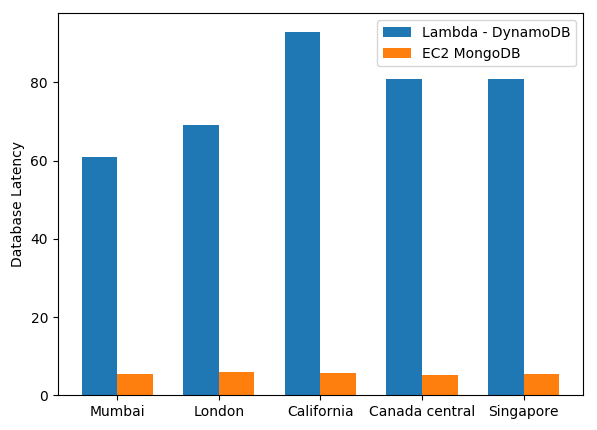
\includegraphics[height=10cm]{Images/1.png}
\caption{Huge difference between lambda and mongoDB}
\end{figure}

\subsection{Analysis}

\begin{itemize}
    \item The latency seen in FaaS is much greater than that in IaaS (approximately 6 times larger).
    \item This latency is too large (greater than 60 ms). Usually 50 ms is tolerable (Ex: in AR/VR applications)
    \item This is just a vanilla setup, the latencies are bound to increase when lambda and database are in different locations.
    \item This calls for some kind of caching mechanism which is going to be the heart of subsequent experiments.
\end{itemize}

\section{Clients spread across the globe}

In this experiment, we study latency and billing differences in invoking lambda functions when clients are present in different locations.

\subsection{Experimental Setup}
\begin{itemize}
    \item Lambda function location : Mumbai
    \item Application is simple web application using DynamoDB in the backend
    \item Clients located at India : Mumbai, USA : North California, Europe : London, Australia : Sidney, Japan : Tokyo.
    \item Used EC2 instances at different locations to emulate clients.
    \item Used AWS API gateway to expose lambda function URLs
    \item Compared 2 types of requests : POST and GET
\end{itemize}

Hypothesis : It should be different across locations due to different number of hops be across locations.

\subsection{Results}

\begin{figure}[ht]
\centering
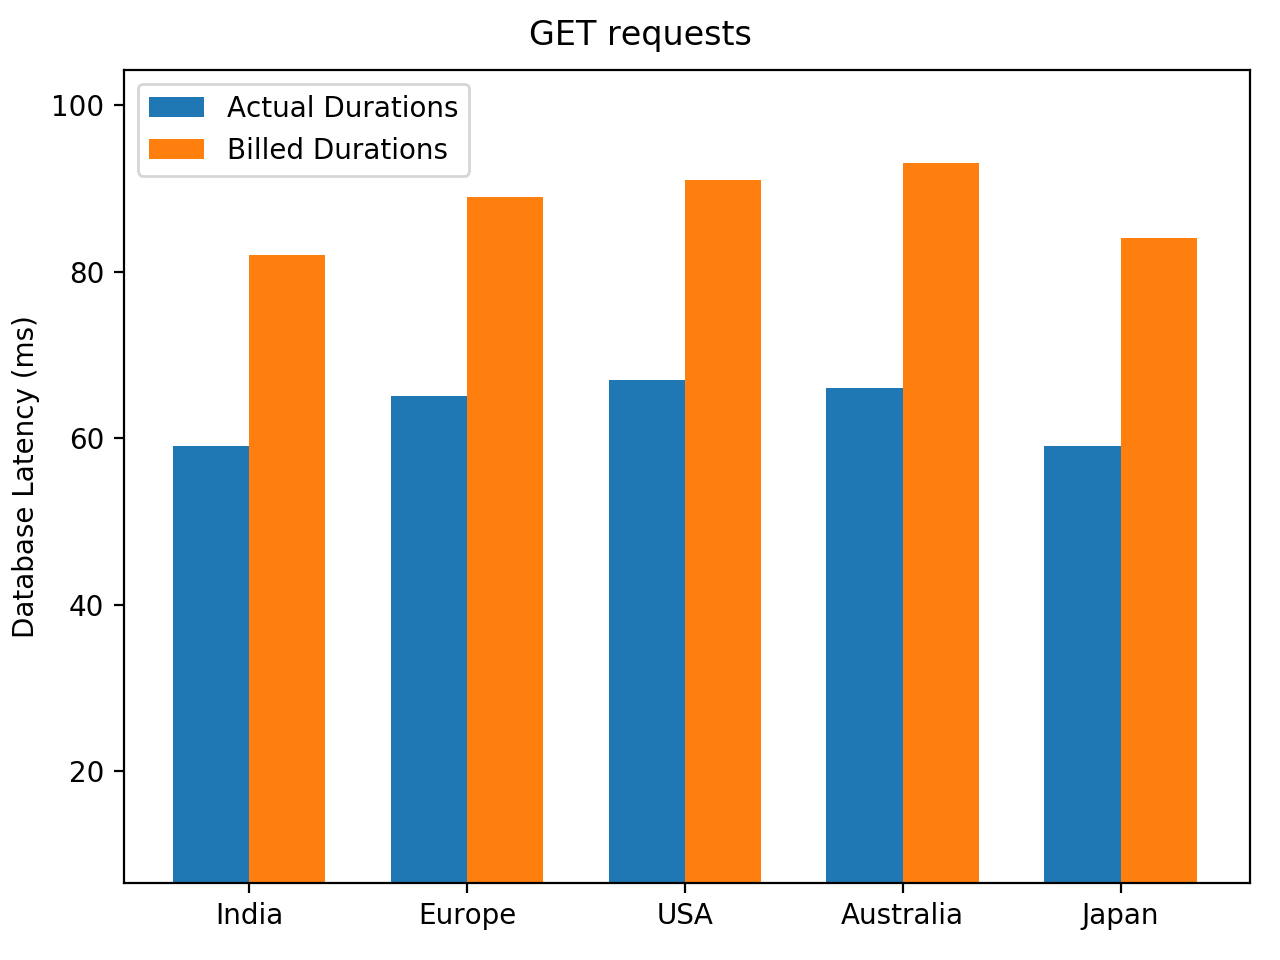
\includegraphics[height=10cm]{Images/2get.png}
\caption{Uniform difference between actual duration and billed duration}
\end{figure}

\begin{figure}[ht]
\centering
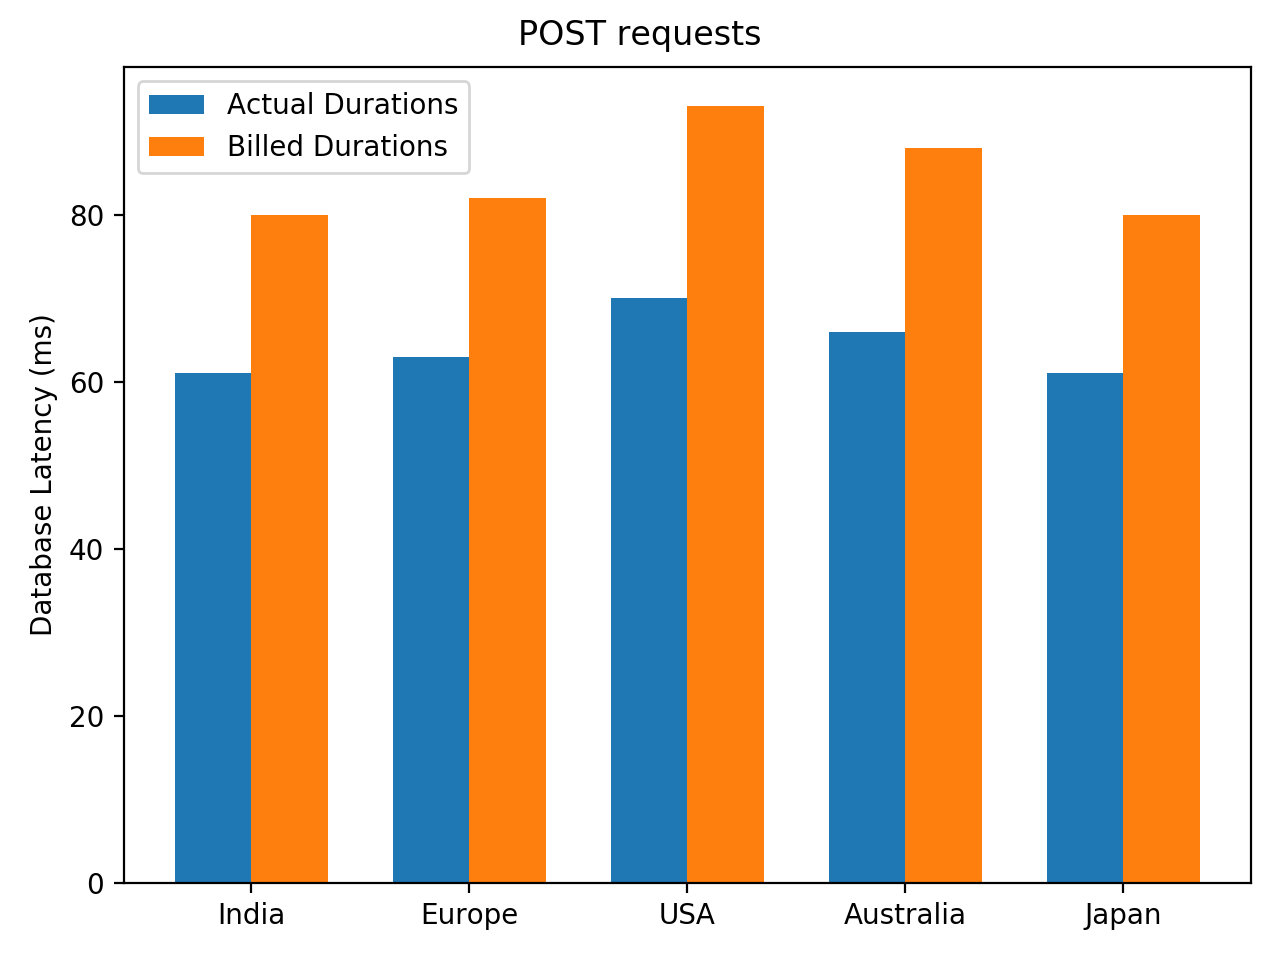
\includegraphics[height=10cm]{Images/2post.png}
\caption{Almost Similar lambda runtimes across clients}
\end{figure}

\subsection{Analysis}

\begin{itemize}
    \item The locations of client don’t affect the running time of lambda functions.
    \item The billed durations and actual duration of making a DB call is uniform across different client locations.
    \item The billed durations and actual duration do not differ much for GET and POST requests.
    \item This suggests that the client TCP connections are actually handled by API gateway exposing the lambda functions through URLs.
    \item The lambda function only receives the parameters, executes and returns the result. The client location is unknown to it.
    \item We also observe that the latency is uniformly high across different client locations.
    \item The difference between billed duration and actual DB call duration is very low compared to actual DB call duration, meaning that major portion of runtime is wasted while waiting for DB calls to return.
    \item This suggests that we can make the DB calls faster by placing some cache in between for read (GET) requests or delegating it to other lambda functions for write (POST) requests.
\end{itemize}

\section{Cache between lambda and DB}

In this experiment, we study latency differences of using various cache between lambda and DB.

\subsection{Experimental Setup}
\begin{itemize}
    \item AWS lambda
    \item For comparisons used DynamoDB directly, used Global variables as cache, used redis cache as cache
\end{itemize}

Hypothesis : Using global variables should give least latency as the variables would be stored nearest to lambda.

\subsection{Results}

\begin{figure}[ht]
\centering
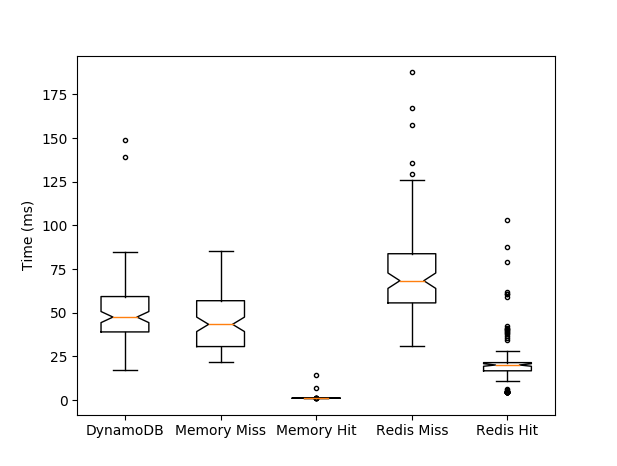
\includegraphics[height=10cm]{Images/3.png}
\caption{Global variable cache hit latency is negligible}
\end{figure}

\subsection{Analysis}

\begin{itemize}
    \item The latency seen with global variable cache is negligible.
    \item The latency in order from best to worst is global cache hit, redis cache hit, global cache miss, direct DynamoDB access and then redis cache miss.
    \item The global variables works best but it comes with a constraint. We observed that the global variables are shared only across lambda invocations within same sessions. After a cold start, the global variables are reset.
    \item Also, this problem would come when load is high and multiple containers are running at the same time. The lambda invocations in 2 different containers would be unknown to each other.
    \item Hence, it makes sense to delegate read calls for lambda too.
\end{itemize}

\section{Nested Lambda}

Here, we analyse the latency incurred when calling one lambda from another lambda.

\subsection{Experimental Setup}
\begin{itemize}
    \item AWS lambda
    \item Used a vanilla function for inner lambda
    \item Outer lambda invokes inner lambda synchronously
    \item Both lambda functions deployed at same location
\end{itemize}

Hypothesis : As the lambda functions are deployed at same location, the latency between calling one lambda from another should be negligible.

\subsection{Results}

\begin{figure}[ht]
\centering
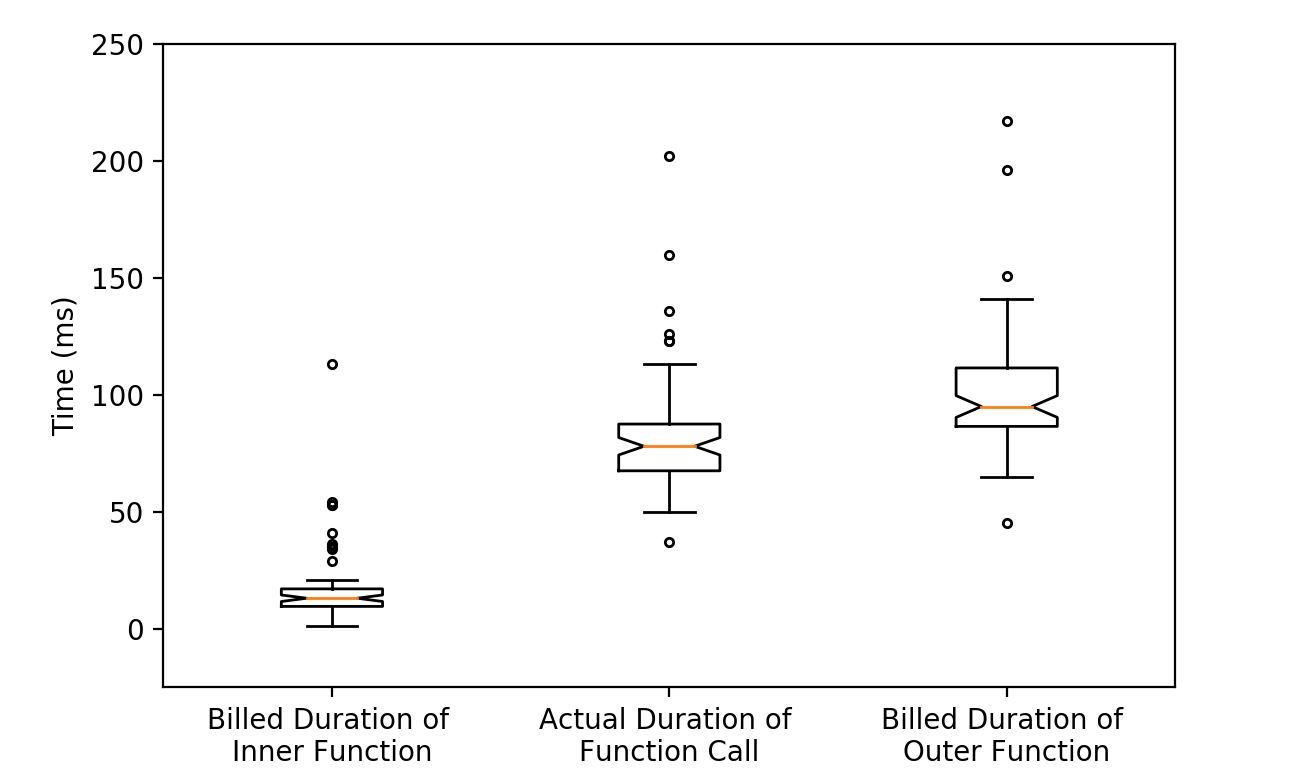
\includegraphics[height=10cm]{Images/4nested.png}
\caption{The billed duration of inner function is negligible but the actual duration of function call inside outer function is very high}
\end{figure}

\subsection{Analysis}

\begin{itemize}
    \item Billed duration of inner function is negligible as it is a vanilla function.
    \item The actual duration of function call seen inside outer function is very large. 
    \item Note that this duration will increase if there is a cache miss inside inner function during read operations.
    \item The actual duration is comparable to that of a DB call (approx 60 ms). 
    \item This suggests that some kind of queuing of requests is taking place with these invocations. 
    \item This also says that nested lambda doesn’t yield much benefit for read operations.
    \item Even though this is not beneficial for DB read operations, nested lambda is beneficial for write operations, when outer function can call inner function asynchronously and doesn’t have to wait for it to return.
    \item In the next experiment we will be seeing how latency is affected on cascading multiple lambdas at different levels.
\end{itemize}

\section{Cascaded Lambda}

Here, we analyse the latency incurred when calling nested lambda at multiple levels.

\subsection{Experimental Setup}
\begin{itemize}
    \item AWS lambda
    \item Used DB write at the innermost lambda
    \item Outer lambda invokes inner lambda synchronously
    \item All lambda functions deployed at same location
\end{itemize}

Hypothesis : As the lambda functions are deployed at same location, the latency between calling one lambda from another should be uniform.

\subsection{Results}

\begin{figure}[ht]
\centering
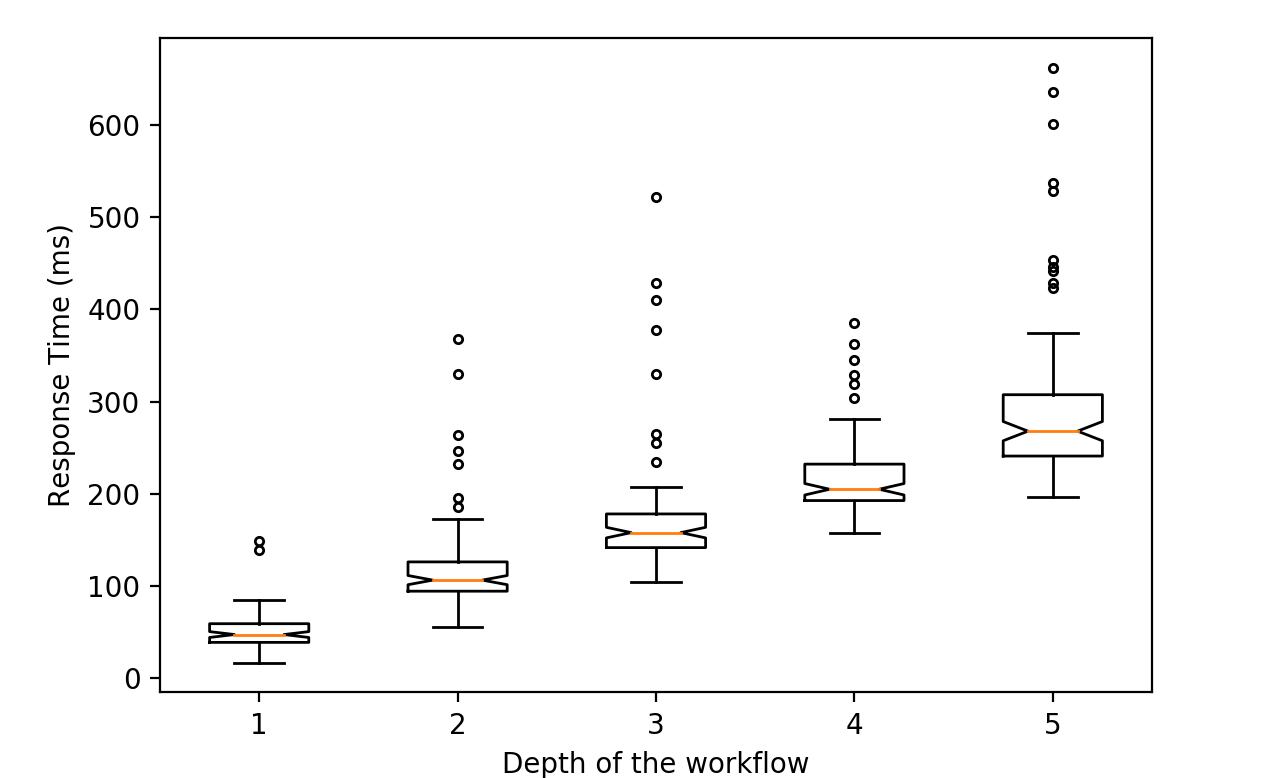
\includegraphics[height=10cm]{Images/5.png}
\caption{The latency of nested functions increases linearly with levels}
\end{figure}

\subsection{Analysis}

\begin{itemize}
    \item As we can see the nested lambda latency increases linearly across the levels.
    \item Using this information, we can increase the performance of an application using cascaded lambda by running a single lambda with all its components instead of running them one after the other.
    \item The uniform difference across different levels of lambda also strengthens the hypothesis that this latency is governed by the queuing delay at the location of deployment. 
    \item Hence, it's important to know what kind of queuing mechanism is in use.
    \item By calling same function recursively, we may be able to overcome the constraint of limited running time.
\end{itemize} 
%% Conçlusion and Future Works. 
% Chapter Template

\chapter{Conclusion and Future Works} % Main chapter title

\label{Chapter 6} % Change X to a consecutive number; for referencing this chapter elsewhere, use \ref{ChapterX}

\lhead{Chapter 6. \emph{Conclusion and Future Works}} % Change X to a consecutive number; this is for the header on each page - perhaps a shortened title

\section{Conclusion}

In this project, we did many analysis regarding latency in serverless frameworks which lead us to following conclusions :

\begin{itemize}
    \item Even though serverless has so many benefits, performance wise it still lags behind traditional approaches.
    \item Experiments done in this project give us important insights on working of serverless platforms, specifically AWS lambda.
    \item Shared global variables provide an easy way of caching but we need to find some turnaround for sharing these variables across runtimes.
    \item We also observe that the 2 functions had individual cold starts, this implies that they are running in separate runtimes.
    \item Multiple lambda functions can be cascaded to overcome time constraints for time-intensive applications.
    \item Multiple lambda functions can be combined if the series of lambda functions to be used is known beforehand to reduce response time.
    \item There is scope for further evolution of serverless architectures by sharing runtimes.
\end{itemize}

\section{Future Works}

In future we would like to achieve the following objectives :
\begin{enumerate}
    \item We would like to study what kind of queuing mechanisms is being used for these invocations and suggest methods to improve latency.
    \item Current platforms use separate runtimes for individual functions. We would like to explore whether we can share this runtime across separate functions. This would also mitigate the problem of cold start and the increased response time due to queuing.
\end{enumerate} 
%\input{Chapters/Chapter7} 

%----------------------------------------------------------------------------------------
%	THESIS CONTENT - APPENDICES
%----------------------------------------------------------------------------------------

\addtocontents{toc}{\vspace{2em}} % Add a gap in the Contents, for aesthetics

% Related Works - Basically, literature survey
% 10 related papers - each paper 6-7 lines explaining what they have done
% Try to put their comparison in a table format
% Research gap : what is missing in these papers

% Chapter Template

\chapter{Related Works} %

\label{Chapter 2} % Change X to a consecutive number; for referencing this chapter elsewhere, use \ref{ChapterX}

\lhead{Chapter 2. \emph{Related Works}} % Change X to a consecutive number; this is for the header on each page - perhaps a shortened title

%----------------------------------------------------------------------------------------
%	SECTION 1
%---------------------------------------------------------------------------------------
\section{Literature Survey}

Here, we discuss the work done in the past.

In \cite{openlambda}, the authors present OpenLambda, a new, open-source platform for building next-generation web services and applications in the burgeoning model of serverless computation. They have described the key aspects of serverless computation, and present numerous research challenges that must be addressed in the design and implementation of such systems. They also did a brief study of current web applications, so as to better motivate some aspects of serverless application construction.

Akkus et al \cite{Akkus_Sand_Usenix_2018} present SAND, a new serverless computing
system that provides lower latency, better resource effi-
ciency and more elasticity than existing serverless plat-
forms. To achieve these properties, SAND introduces two
key techniques: 1) application-level sandboxing, and 2)
a hierarchical message bus. We have implemented and
deployed a complete SAND system. Our results show 
that SAND outperforms the state-of-the-art serverless plat-
forms significantly. For example, in a commonly-used image processing application, SAND achieves a 43\%
speedup compared to Apache OpenWhisk.

\subsection{Understanding Ephemeral Storage for Serverless Analytics}

Klimovic et al \cite{ephemeral} in their paper explore the suitability of different cloud storage services (e.g., object stores and distributed caches) as remote storage for serverless analytics. Their analysis leads to key insights to guide the design of an ephemeral cloud storage system, including the performance and cost efficiency of Flash storage for server-less application requirements and the need for a pay- what-you-use storage service that can support the high throughput demands of highly parallel applications.

In \cite{Wang_usenix_2018}, the authors explain how the platforms isolate the functions of different accounts, using either virtual machines or containers, which has important security implications. They characterize performance in terms of scalability, coldstart latency, and resource efficiency, with highlights including that AWS Lambda adopts a bin-packing-like strategy to maximize VM memory utilization, that severe contention between functions can arise in AWS and Azure, and that Google had bugs that allow customers to use resources for free.

\section{Research Gap}

\begin{itemize}
    \item None of the works so far have compared serverless architecture to serverful architecture on the basis of performance.
    \item Even though most of the serverless applications are web applications that involve interaction with database in the backend, only image processing and data analytics applications have been studied at length.
    \item Today, many of the serverless platforms have server farms in various parts of the world, hence, strategic placement of lambda functions and databases becomes an important case study for increasing performance of these applications.
\end{itemize}

% \section{Types of faults}

% \subsection{Crash Faults}

% A replica is said to be crash-faulty if it stops all computation and communication.

% \subsection{Byzantine Faults}

% A replica is said to be Byzantine or non-crash faulty if it acts arbitrarily, but cannot break cryptographic primitives we use (crypto- graphic hashes, MACs, message digests and digital signatures).

% \subsection{Network Faults}

% A network fault is defined as the inability of some correct replicas to communicate with each other in a timely manner, that is, when a message exchanged between two correct replicas cannot be delivered and processed within delay $\Delta$, known to all replicas.


% \paragraph{Literature Survey}

% This is a sample. Write about referred papers. Cite like this \citep{nip2010cyclic}. Another example would be this \citep{nip2010extremely}. More citations like this \citep{bird2004evaluating}, \citep {tremblay2003seismic} and \citep {alhamaydeh2016key}.

% \paragraph{Research gaps}
% Typically include research gaps for your study. 
% \paragraph{Objective}
% Similarly objectives of study. 
% \paragraph{Scope}
% Define scope of study. 
% \paragraph{An algorithm}
% How you could refer to figures: This is an example. (Refer \ref{fig5}). You can add equations like this Eq. (\ref{eq1})
% \begin{equation}
% \label{eq1}
%   SDR = sd(T) - \sum_{i}\frac{{T}_{i}}{|T|}\times sd({T}_{i})
% \end{equation}

% \begin{figure}[]
% \centering
% \includegraphics[height=7cm]{splits.png}
% \caption{Splitting of the input space (X1 x X2) by M5' model tree algorithm}
% \label{fig5}
% \end{figure}

% \section{Adding another section}
% You can show a lot of figures together like these Figures \ref{fig61}, \ref{fig62}, \ref{fig63} below.
% \begin{figure} [!htbp]
% \centering    
% \subfigure[Caption1]{\label{fig61}\includegraphics[width=42mm]{data1.png}}
% \subfigure[Caption2]{\label{fig62}\includegraphics[width=42mm]{data2.png}}
% \subfigure[Caption3]{\label{fig63}\includegraphics[width=42mm]{data3.png}}
% \caption{Figures sample}
% \end{figure}
% You can add lists into the text like this. 
% \begin{itemize}
% \settowidth{\leftmargin}{{\Large$\square$}}\advance\leftmargin\labelsep
% \itemsep3pt\relax
% \renewcommand\labelitemi{{\lower1pt\hbox{\small$\square$}}}
% \item	Some sample text item 1. 
% \item You may refer to tables \ref{tab1} 
% \item Or figures \ref{fig61}
% \end{itemize}

% Tables can be added like this
% \begin{table}[!htbp]
% \centering
% \caption{Sample table}
% \label{tab1}
% \begin{tabular}{llll}

% \hline
% Column 1 & Column 2 & Column 3       \\\hline
% 1         & Data1 & 13.41179 & 0.9492839 \\
% 2            & Data2 & 13.39824 & 0.9492952\\\hline
% \end{tabular}
% \end{table}




\addtocontents{toc}{\vspace{2em}} % Add a gap in the Contents, for aesthetics

% Proposal / Objective
% Motivation

% Chapter Template

\chapter{Objective} % Main chapter title

\label{Chapter 3} % Change X to a consecutive number; for referencing this chapter elsewhere, use \ref{ChapterX}

\lhead{Chapter 3. \emph{Objective}} % Change X to a consecutive number; this is for the header on each page - perhaps a shortened title

%----------------------------------------------------------------------------------------
%	SECTION 1
%---------------------------------------------------------------------------------------
\section{Problem Motivation}

\begin{itemize}
    \item Serverless platforms isolate and execute functions in separate containers, and do not exploit the interactions among functions for performance. These practices lead to high startup delays for function executions and inefficient resource usage.
    \item Many of such applications interact with a database in the backend. Even if we ignore the startup delays, in the normal executions also when the container is warm, the delay is 5 times more as compared to a dedicated server.
    \item This delay increases even more when the database and the lambda function is not placed in the same location.
\end{itemize}



\section{Problem Statement}

\begin{itemize}
    \item Characterizing latency in serverless architectures with respect to database applications and strategies to improve it.
    \item Improving performance by placing cache optimally across lambda.
\end{itemize}

\section{Contributions}

We contribute by studying following latency analysis :

\begin{itemize}
    \item Between traditional server architectures IaaS and serverless architectures FaaS.
    \item When same lambda function is accessed by clients from multiple locations.
    \item Between different type of requests like GET requests (read) and POST requests (write) when deployed using lambda.
    \item Between different type of caching like in-memory caching and external caching.
    \item When one lambda calls another lambda (Nested lambda).
    \item When multiple lambda functions are cascaded at different depths.
\end{itemize}

\addtocontents{toc}{\vspace{2em}} % Add a gap in the Contents, for aesthetics

% Discussion - Discuss the issues that you have got in the system, an idea about how you are trying to solve those. 
% Chapter Template

\chapter{Proposed Model} % Main chapter title

\label{Chapter 4} % Change X to a consecutive number; for referencing this chapter elsewhere, use \ref{ChapterX}

\lhead{Chapter 4. \emph{Proposed Model}} % Change X to a consecutive number; this is for the header on each page - perhaps a shortened title

In our experiments, we saw that difference in latencies when using traditional approaches and while using serverless architecture is huge even with cold starts ignored. This difference paves way for solutions where we can minimize this difference and the foremost technique that comes to our mind is caching. Hence, we propose different kinds of caching and through our experiments try to determine how much improvement can we gain with caching.

\section{POST requests (write calls)}

With write calls, the easiest way to achieve performance is by delegating the actual writing to another lambda function asynchronously and spend time only in doing sanity checks of the data to be written. The only problem that will arise is the problem of consistency which will anyway be maintained by the database. This can be done easily by declaring a separate lambda function whose only job is to write data to the database and the actual lambda function can call this function asynchronously without waiting for it to return.

\section{GET requests (read calls)}

With read calls, its imperative to use cache as the data needs to be fetched from the database. If the cache is warm (cache hit) then the response time would be very low but if the cache is cold (cache miss or cache is stale) then the response time would be more as the time spent in fetching data from the database will affect the response time. But usually the performance of these caches is determined when the same data is requested again and again. In this project, we have tried to analyse how different types of cache affect the performance of these function calls. Different types of cache studied is :

\begin{itemize}
    \item External cache : Here, by external we mean external to the lambda runtime. For this experiment, we use redis as an in-memory cache store between lambda function and the database and we place all the three in same location.
    \item Internal cache : Here, by internal we mean internal to the runtime executing the lambda function. AWS lambda provides a feature where global variables are shared between different function calls of the same lambda function. But, this feature comes with its own constraints like the global variables are shared between only those function calls which are sharing the session. Once, the container is stopped, session is closed, all the data stored in the global variables is lost. This is also true when multiple sessions are running at the same time when load is very high. These sessions would be working on separate global variables. Not only this, there is a constraint on the runtime of lambda functions and if the calls are not frequent then the cache won't stay warm. A workaround to this is that again delegate the job of fetching data to another lambda function, which also invokes another of its instance just for the sake of keeping cache warm and then returns. But, this technique can only work if latency of calling another lambda function in a nested way is very low.
\end{itemize}

In our experiments, we would be verifying if above approaches are possible and if so how much performance improvement do they give.

\addtocontents{toc}{\vspace{2em}} % Add a gap in the Contents, for aesthetics

% Discussion - Discuss the issues that you have got in the system, an idea about how you are trying to solve those. 
% Chapter Template

\chapter{Experiments, Results and Observations} % Main chapter title

\label{Chapter 5} % Change X to a consecutive number; for referencing this chapter elsewhere, use \ref{ChapterX}

\lhead{Chapter 5. \emph{Experiments, Results and Analysis}} % Change X to a consecutive number; this is for the header on each page - perhaps a shortened title

We have used Amazon AWS as serverless platform for our analysis as it is the most popular public serverless platform in use today (Source : Google Trends).

Also, our experiments mainly focus on web-based applications that use a database in the backend for which we have used AWS DynamoDB.

In addition to that, we have used AWS API gateway to generate URLs for testing purposes for exposing the lambda functions to the public.

We perform following experiments in the project :

\begin{enumerate}
    \item Traditional (IaaS) vs Serverless (FaaS)
    \item Serverless : clients spread across the globe
    \item Using cache between lambda and database
    \item Nested lambda latency
    \item Cascading lambda with different levels
\end{enumerate}

\section{IaaS vs FaaS}

In this experiment, we study latency differences of deploying a web application on dedicated servers and that with lambda functions.

\subsection{Experimental Setup}
\begin{itemize}
    \item IaaS : EC2 instances with MongoDB on backend
    \item FaaS : AWS lambda with AWS DynamoDB on backend
    \item Both lambda and DynamoDB placed at same location
    \item Locations studied : Mumbai, London, California, Canada Central, Singapore
\end{itemize}

Hypothesis : It should be same as DB and lambda deployed in the same location as EC2.

\subsection{Results}

\begin{figure}[ht]
\centering
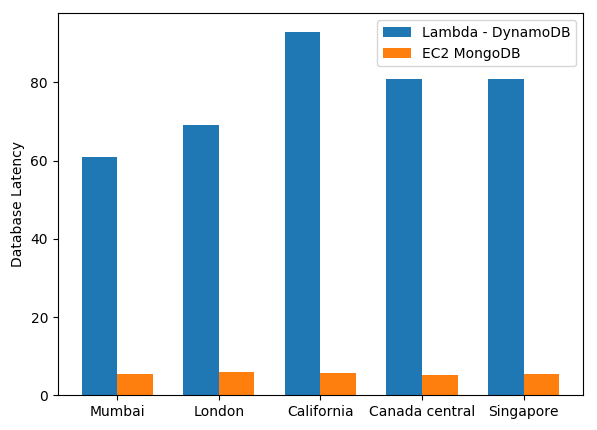
\includegraphics[height=10cm]{Images/1.png}
\caption{Huge difference between lambda and mongoDB}
\end{figure}

\subsection{Analysis}

\begin{itemize}
    \item The latency seen in FaaS is much greater than that in IaaS (approximately 6 times larger).
    \item This latency is too large (greater than 60 ms). Usually 50 ms is tolerable (Ex: in AR/VR applications)
    \item This is just a vanilla setup, the latencies are bound to increase when lambda and database are in different locations.
    \item This calls for some kind of caching mechanism which is going to be the heart of subsequent experiments.
\end{itemize}

\section{Clients spread across the globe}

In this experiment, we study latency and billing differences in invoking lambda functions when clients are present in different locations.

\subsection{Experimental Setup}
\begin{itemize}
    \item Lambda function location : Mumbai
    \item Application is simple web application using DynamoDB in the backend
    \item Clients located at India : Mumbai, USA : North California, Europe : London, Australia : Sidney, Japan : Tokyo.
    \item Used EC2 instances at different locations to emulate clients.
    \item Used AWS API gateway to expose lambda function URLs
    \item Compared 2 types of requests : POST and GET
\end{itemize}

Hypothesis : It should be different across locations due to different number of hops be across locations.

\subsection{Results}

\begin{figure}[ht]
\centering
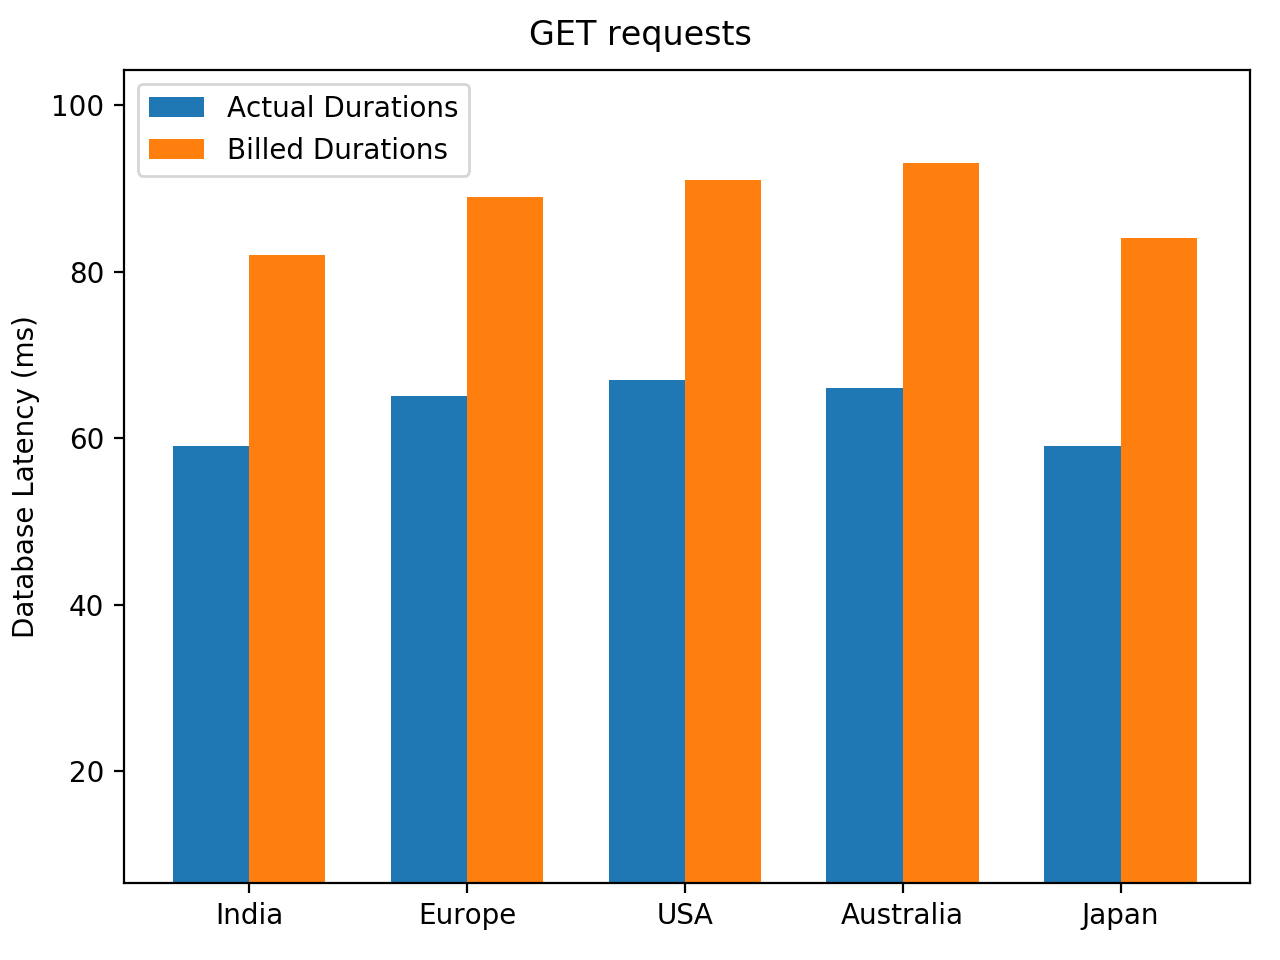
\includegraphics[height=10cm]{Images/2get.png}
\caption{Uniform difference between actual duration and billed duration}
\end{figure}

\begin{figure}[ht]
\centering
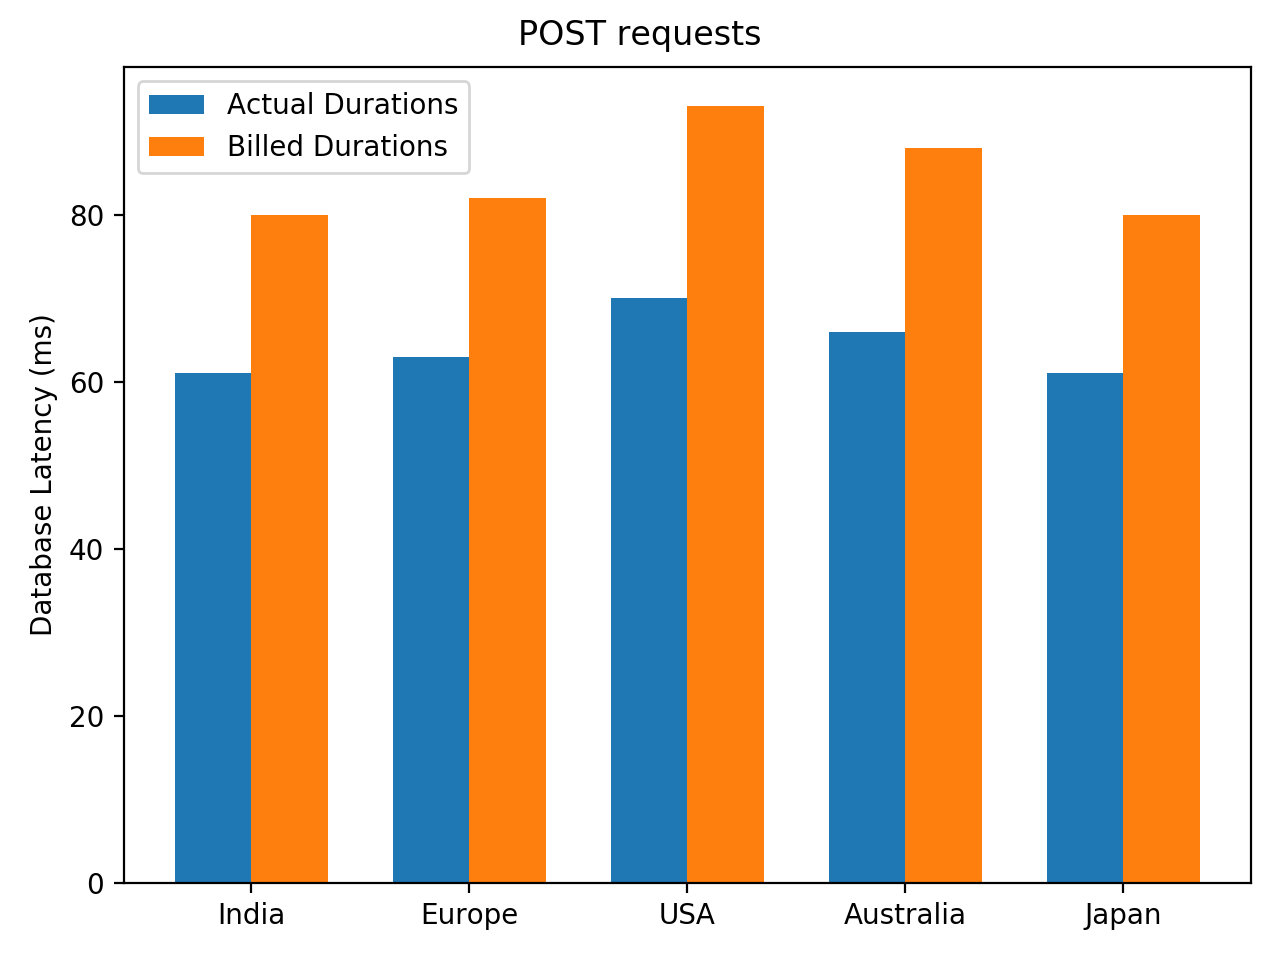
\includegraphics[height=10cm]{Images/2post.png}
\caption{Almost Similar lambda runtimes across clients}
\end{figure}

\subsection{Analysis}

\begin{itemize}
    \item The locations of client don’t affect the running time of lambda functions.
    \item The billed durations and actual duration of making a DB call is uniform across different client locations.
    \item The billed durations and actual duration do not differ much for GET and POST requests.
    \item This suggests that the client TCP connections are actually handled by API gateway exposing the lambda functions through URLs.
    \item The lambda function only receives the parameters, executes and returns the result. The client location is unknown to it.
    \item We also observe that the latency is uniformly high across different client locations.
    \item The difference between billed duration and actual DB call duration is very low compared to actual DB call duration, meaning that major portion of runtime is wasted while waiting for DB calls to return.
    \item This suggests that we can make the DB calls faster by placing some cache in between for read (GET) requests or delegating it to other lambda functions for write (POST) requests.
\end{itemize}

\section{Cache between lambda and DB}

In this experiment, we study latency differences of using various cache between lambda and DB.

\subsection{Experimental Setup}
\begin{itemize}
    \item AWS lambda
    \item For comparisons used DynamoDB directly, used Global variables as cache, used redis cache as cache
\end{itemize}

Hypothesis : Using global variables should give least latency as the variables would be stored nearest to lambda.

\subsection{Results}

\begin{figure}[ht]
\centering
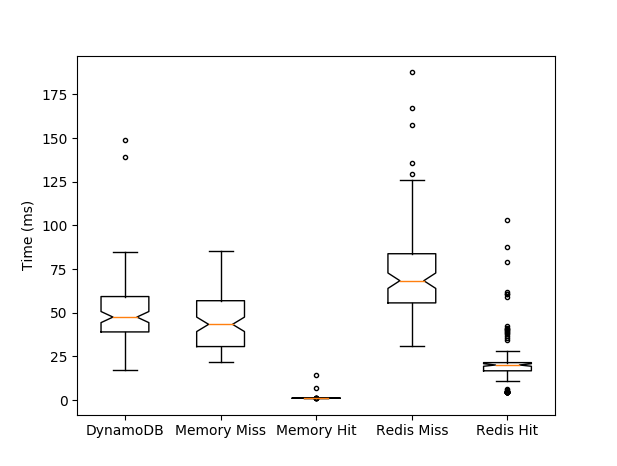
\includegraphics[height=10cm]{Images/3.png}
\caption{Global variable cache hit latency is negligible}
\end{figure}

\subsection{Analysis}

\begin{itemize}
    \item The latency seen with global variable cache is negligible.
    \item The latency in order from best to worst is global cache hit, redis cache hit, global cache miss, direct DynamoDB access and then redis cache miss.
    \item The global variables works best but it comes with a constraint. We observed that the global variables are shared only across lambda invocations within same sessions. After a cold start, the global variables are reset.
    \item Also, this problem would come when load is high and multiple containers are running at the same time. The lambda invocations in 2 different containers would be unknown to each other.
    \item Hence, it makes sense to delegate read calls for lambda too.
\end{itemize}

\section{Nested Lambda}

Here, we analyse the latency incurred when calling one lambda from another lambda.

\subsection{Experimental Setup}
\begin{itemize}
    \item AWS lambda
    \item Used a vanilla function for inner lambda
    \item Outer lambda invokes inner lambda synchronously
    \item Both lambda functions deployed at same location
\end{itemize}

Hypothesis : As the lambda functions are deployed at same location, the latency between calling one lambda from another should be negligible.

\subsection{Results}

\begin{figure}[ht]
\centering
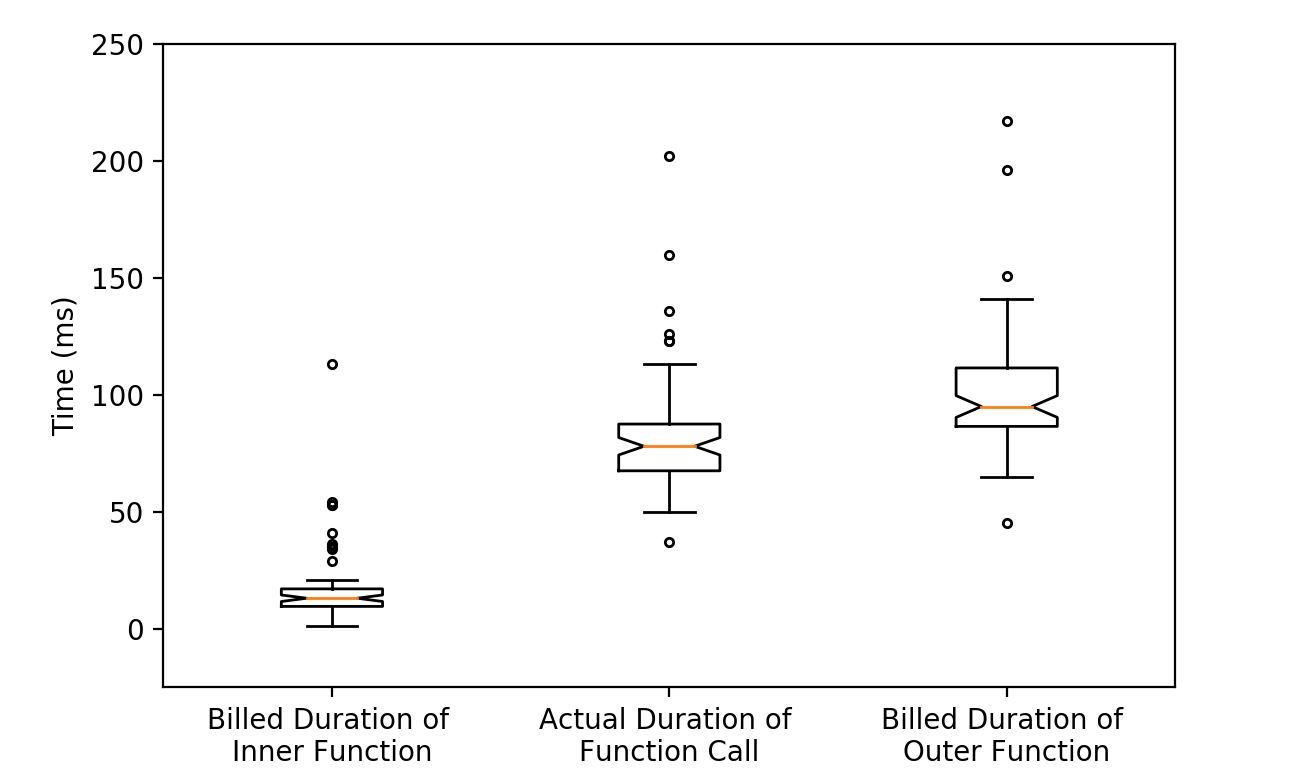
\includegraphics[height=10cm]{Images/4nested.png}
\caption{The billed duration of inner function is negligible but the actual duration of function call inside outer function is very high}
\end{figure}

\subsection{Analysis}

\begin{itemize}
    \item Billed duration of inner function is negligible as it is a vanilla function.
    \item The actual duration of function call seen inside outer function is very large. 
    \item Note that this duration will increase if there is a cache miss inside inner function during read operations.
    \item The actual duration is comparable to that of a DB call (approx 60 ms). 
    \item This suggests that some kind of queuing of requests is taking place with these invocations. 
    \item This also says that nested lambda doesn’t yield much benefit for read operations.
    \item Even though this is not beneficial for DB read operations, nested lambda is beneficial for write operations, when outer function can call inner function asynchronously and doesn’t have to wait for it to return.
    \item In the next experiment we will be seeing how latency is affected on cascading multiple lambdas at different levels.
\end{itemize}

\section{Cascaded Lambda}

Here, we analyse the latency incurred when calling nested lambda at multiple levels.

\subsection{Experimental Setup}
\begin{itemize}
    \item AWS lambda
    \item Used DB write at the innermost lambda
    \item Outer lambda invokes inner lambda synchronously
    \item All lambda functions deployed at same location
\end{itemize}

Hypothesis : As the lambda functions are deployed at same location, the latency between calling one lambda from another should be uniform.

\subsection{Results}

\begin{figure}[ht]
\centering
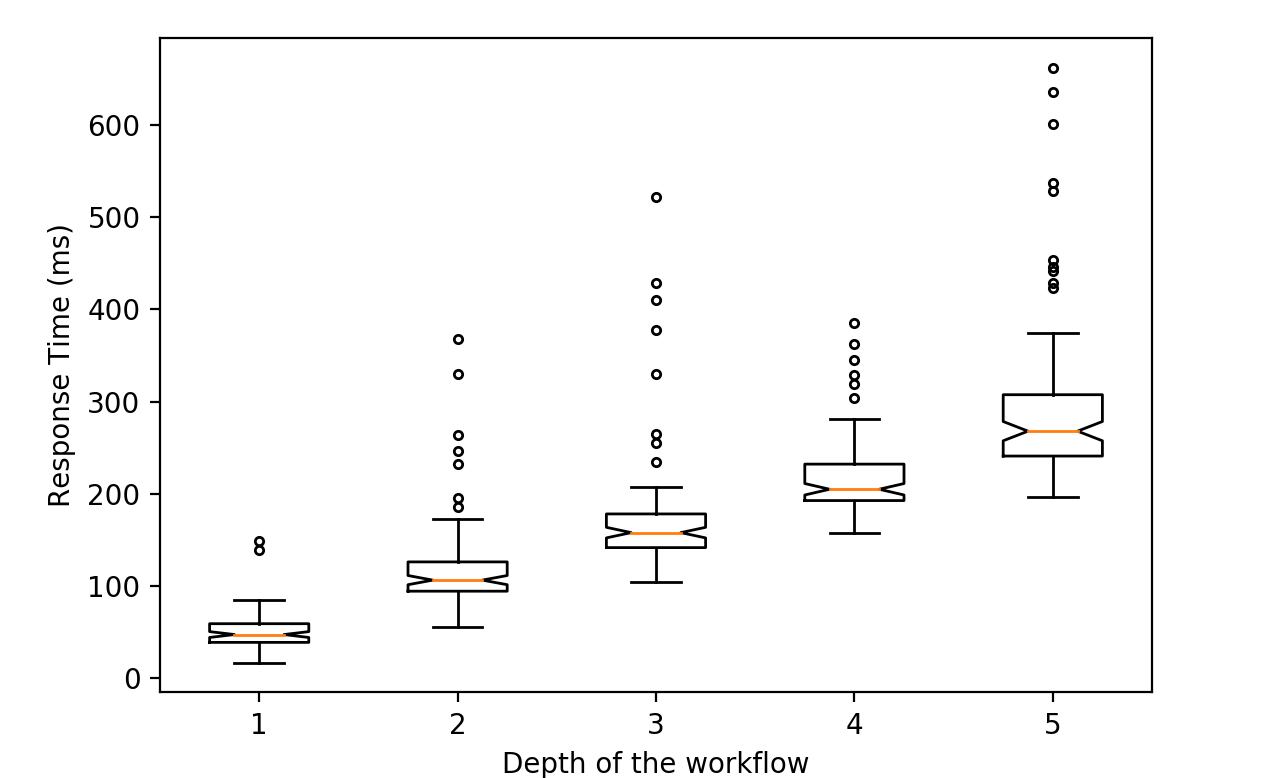
\includegraphics[height=10cm]{Images/5.png}
\caption{The latency of nested functions increases linearly with levels}
\end{figure}

\subsection{Analysis}

\begin{itemize}
    \item As we can see the nested lambda latency increases linearly across the levels.
    \item Using this information, we can increase the performance of an application using cascaded lambda by running a single lambda with all its components instead of running them one after the other.
    \item The uniform difference across different levels of lambda also strengthens the hypothesis that this latency is governed by the queuing delay at the location of deployment. 
    \item Hence, it's important to know what kind of queuing mechanism is in use.
    \item By calling same function recursively, we may be able to overcome the constraint of limited running time.
\end{itemize}

\addtocontents{toc}{\vspace{2em}} % Add a gap in the Contents, for aesthetics

% Conçlusion and Future Works. 
% Chapter Template

\chapter{Conclusion and Future Works} % Main chapter title

\label{Chapter 6} % Change X to a consecutive number; for referencing this chapter elsewhere, use \ref{ChapterX}

\lhead{Chapter 6. \emph{Conclusion and Future Works}} % Change X to a consecutive number; this is for the header on each page - perhaps a shortened title

\section{Conclusion}

In this project, we did many analysis regarding latency in serverless frameworks which lead us to following conclusions :

\begin{itemize}
    \item Even though serverless has so many benefits, performance wise it still lags behind traditional approaches.
    \item Experiments done in this project give us important insights on working of serverless platforms, specifically AWS lambda.
    \item Shared global variables provide an easy way of caching but we need to find some turnaround for sharing these variables across runtimes.
    \item We also observe that the 2 functions had individual cold starts, this implies that they are running in separate runtimes.
    \item Multiple lambda functions can be cascaded to overcome time constraints for time-intensive applications.
    \item Multiple lambda functions can be combined if the series of lambda functions to be used is known beforehand to reduce response time.
    \item There is scope for further evolution of serverless architectures by sharing runtimes.
\end{itemize}

\section{Future Works}

In future we would like to achieve the following objectives :
\begin{enumerate}
    \item We would like to study what kind of queuing mechanisms is being used for these invocations and suggest methods to improve latency.
    \item Current platforms use separate runtimes for individual functions. We would like to explore whether we can share this runtime across separate functions. This would also mitigate the problem of cold start and the increased response time due to queuing.
\end{enumerate}

\addtocontents{toc}{\vspace{2em}} % Add a gap in the Contents, for aesthetics

% \input{Chapters/Chapter7}

% \addtocontents{toc}{\vspace{2em}} % Add a gap in the Contents, for aesthetics

% \appendix % Cue to tell LaTeX that the following 'chapters' are Appendices

% % Include the appendices of the thesis as separate files from the Appendices folder
% % Uncomment the lines as you write the Appendices

% % Appendix Template

\chapter{Appendix A} % Main appendix title

\label{AppendixX} % Change X to a consecutive letter; for referencing this appendix elsewhere, use \ref{AppendixX}

\lhead{Appendix X. \emph{Appendix Title Here}} % Change X to a consecutive letter; this is for the header on each page - perhaps a shortened title

Write your Appendix content here.

% %\input{Appendices/AppendixB}
% %\input{Appendices/AppendixC}

% \addtocontents{toc}{} % Add a gap in the Contents, for aesthetics

%\backmatter

%----------------------------------------------------------------------------------------
%	BIBLIOGRAPHY
%----------------------------------------------------------------------------------------
%\nocite{*}
\clearpage

%\addtotoc{Acknowledgements}
%\thispagestyle{plain}


% \chapter{References} % Main chapter title

% \label{References} % Change X to a consecutive number; for referencing this chapter elsewhere, use \ref{ChapterX}

% \lhead{\emph{References}} % Change X to a consecutive number; this is for the header on each page - perhaps a shortened title


%\label{References}

%\btypeout{References}
%\begin{center}{\huge{\textit{Acknowledgements}} \par}\end{center}

%\lhead{\emph{References}} % Change the page header to say "Bibliography"


\addtotoc{Bibliography}

\bibliographystyle{IEEEtran} % Use the "custom" BibTeX style for formatting the Bibliography

\bibliography{Bibliography} % The references (bibliography) information are stored in the file named "Bibliography.bib"

% \begin{enumerate}
%     \item S. Nakamoto, Bitcoin: A Peer-to-Peer Electronic Cash System, 2008.
%     \item S. Liu, P. Viotti, C. Cachin, V. Quéma, M. Vukolic, "XFT: practical fault tolerance beyond crashes", Proc. 12th USENIX OSDI, 2016.
%     \item Y. Gilad, R. Hemo, S. Micali, G. Vlachos, N. Zeldovich, "Algorand: Scaling Byzantine Agreements for Cryptocurrencies", Cryptology ePrint Archive Report 2017/454, 2017.
%     \item https://en.wikipedia.org/wiki/State\_machine\_replication
%     \item https://en.wikipedia.org/wiki/Blockchain
%     \item https://medium.com/@deshpande.pralhad/a-proof-of-stake-blockchain-with-two-native-asset-types-35f643bb3ff3
%     \item https://open.lib.umn.edu/principleseconomics/chapter/25-2-demand-supply-and-equilibrium-in-the-money-market/
%     \item https://medium.com/coinmonks/understanding-proof-of-stake-the-nothing-at-stake-theory-1f0d71bc027
%     \item https://lisk.io/academy/blockchain-basics/how-does-blockchain-work/proof-of-stake
%     \item Cynthia Dwork and Moni Naor. Pricing via processing or combatting junk mail. In 12th Annual International Cryptology Conference, pages 139–147, 1992.
%     \item “Ethereum: A secure decentralised generalised transaction ledger“. G Wood. 2014. cryptopapers.net Ethereum Project Yellow Paper. 223 cites.
%     \item A. Miller, Y. Xia, K. Croman, E. Shi, and D. Song. The Honey Badger of BFT protocols. In Proceedings of the 23rd ACM Conference on Computer and Communications Security (CCS), pages 31–42, Vienna, Austria, Oct. 2016.
%     \item D. Schwartz, N. Youngs, A. Britto, "The ripple protocol consensus algorithm", 2014, [online] Available: https://ripple.com/files/ripple\_consensus\_whitepaper.pdf.
%     \item Elli Androulaki, Artem Barger, Vita Bortnikov, Christian Cachin, Konstantinos Christidis, Angelo De Caro, David Enyeart, Christopher Ferris, Gennady Laventman, Yacov Manevich et al., Hyperledger fabric: A distributed operating system for permissioned blockchains., 2018.
%     \item Brown, R.G. (2018). The Corda Platform: An Introduction. Retrieved 27.10.2018 from https://www.corda.net/content/corda-platform-whitepaper.pdf
%     \item https://medium.com/edchain/a-comparison-between-5-major-blockchain-protocols-b8a6a46f8b1f
% \end{enumerate}

\end{document}  
